\documentclass[14pt,a4paper]{book}

% Използване на български език.
\usepackage[english,bulgarian]{babel}
\usepackage[utf8]{inputenc}

% Използване на графика.
\usepackage[pdftex]{graphicx}

% Използване на PDF-и за кориците.
\usepackage{pdfpages}

% Използване на хедър и футър.
\usepackage{fancyhdr}

% Заглавие.
\title{Блоково програмиране със Scratch и App Inventor}

% Автори.
\author{Тодор Балабанов, Галя Петрова}

% Директория с изображения.
\graphicspath{{images/}}

% Избор на активен език.
\selectlanguage{bulgarian}

% За кавички при цитиране.
\usepackage{dirtytalk}

% Текстове за декорация на страницата в горната и долната част.
\pagestyle{fancy}
\fancyhf{}
\fancyhead[LE,RO]{\thepage}
\fancyhead[RE]{Блоково програмиране със Scratch и App Inventor}
\fancyhead[LO]{Тодор Балабанов, Галя Петрова}
\fancyfoot[LE,RO]{Издателство \say{Образование и Познание}, 2020}

% Дебелина на разделителната линия.
\renewcommand{\headrulewidth}{2pt}
\renewcommand{\footrulewidth}{1pt}

\begin{document}

% Предна корица.
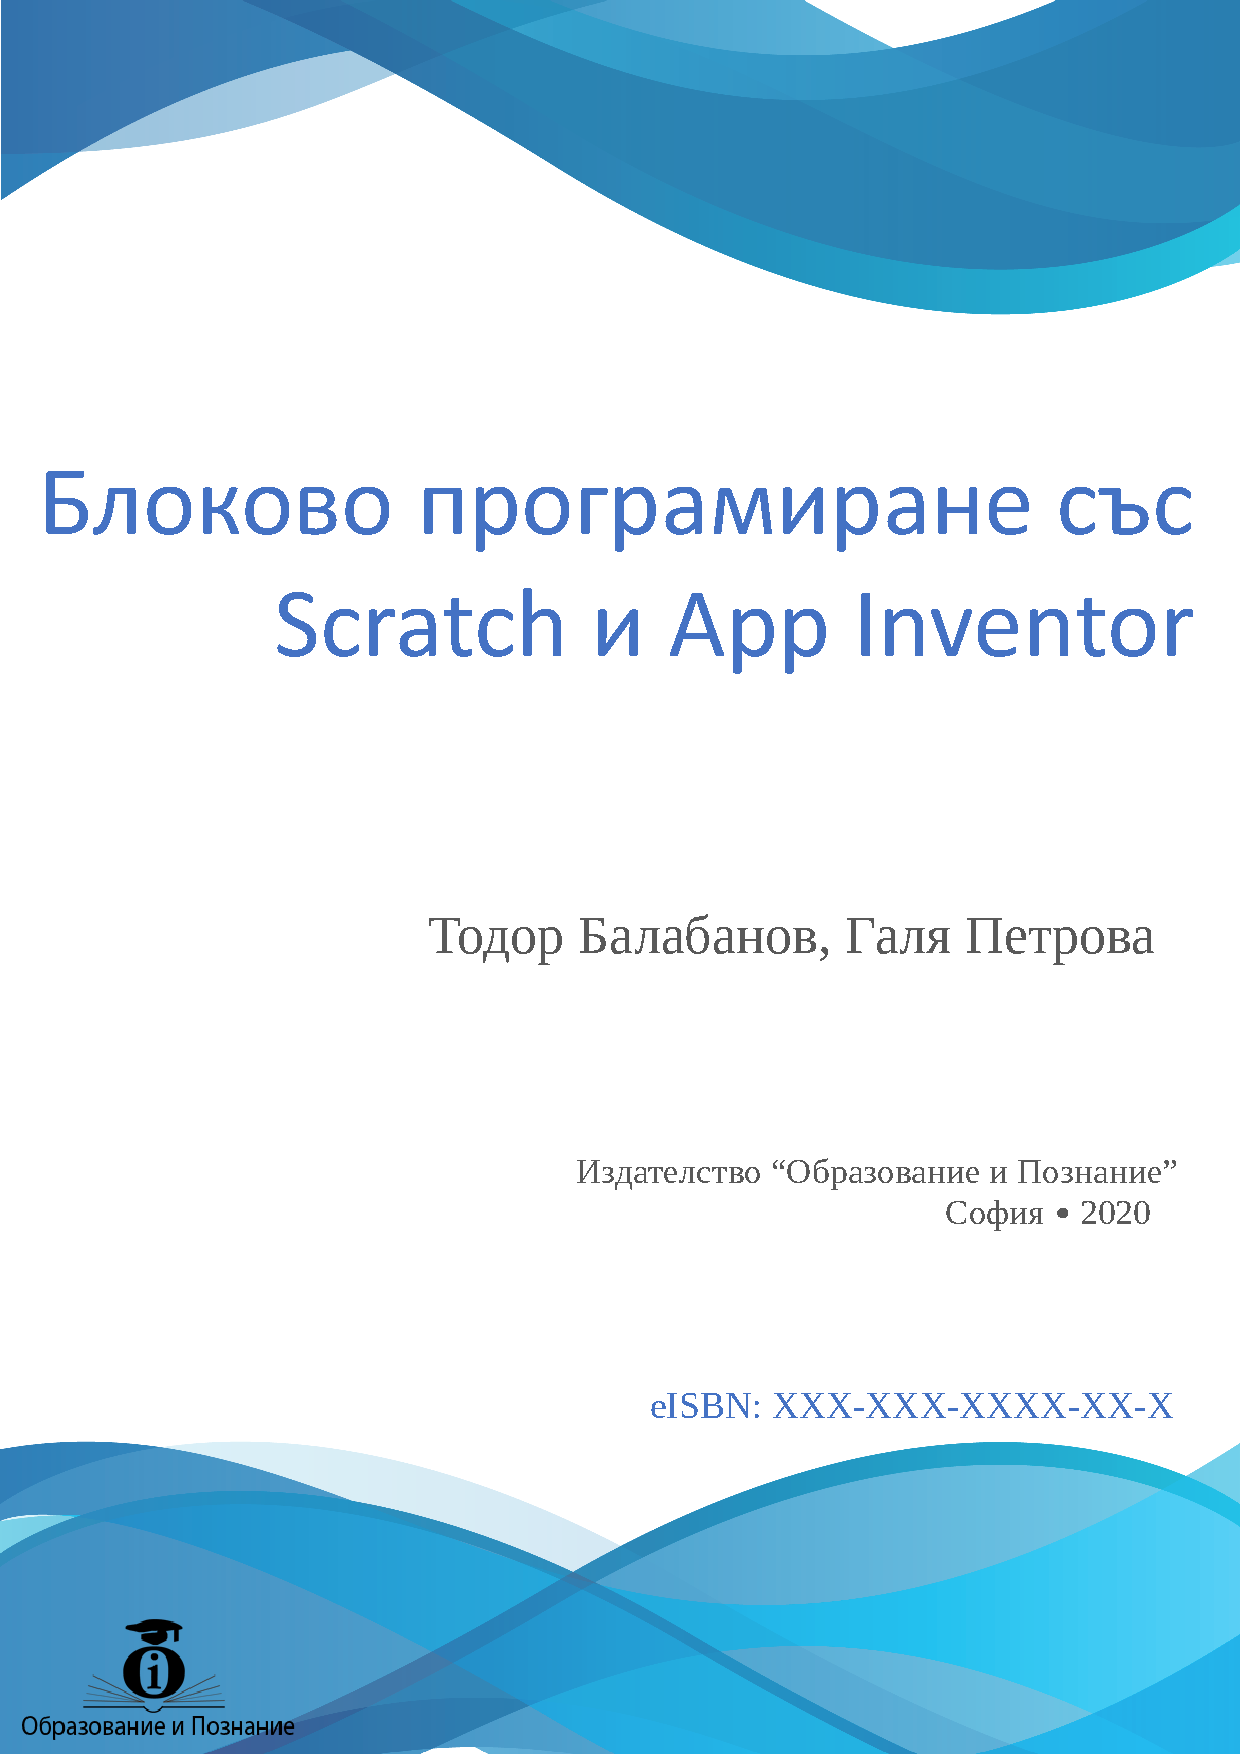
\includepdf[pages={1}]{cover/front}
\thispagestyle{empty}

% Задна корица.
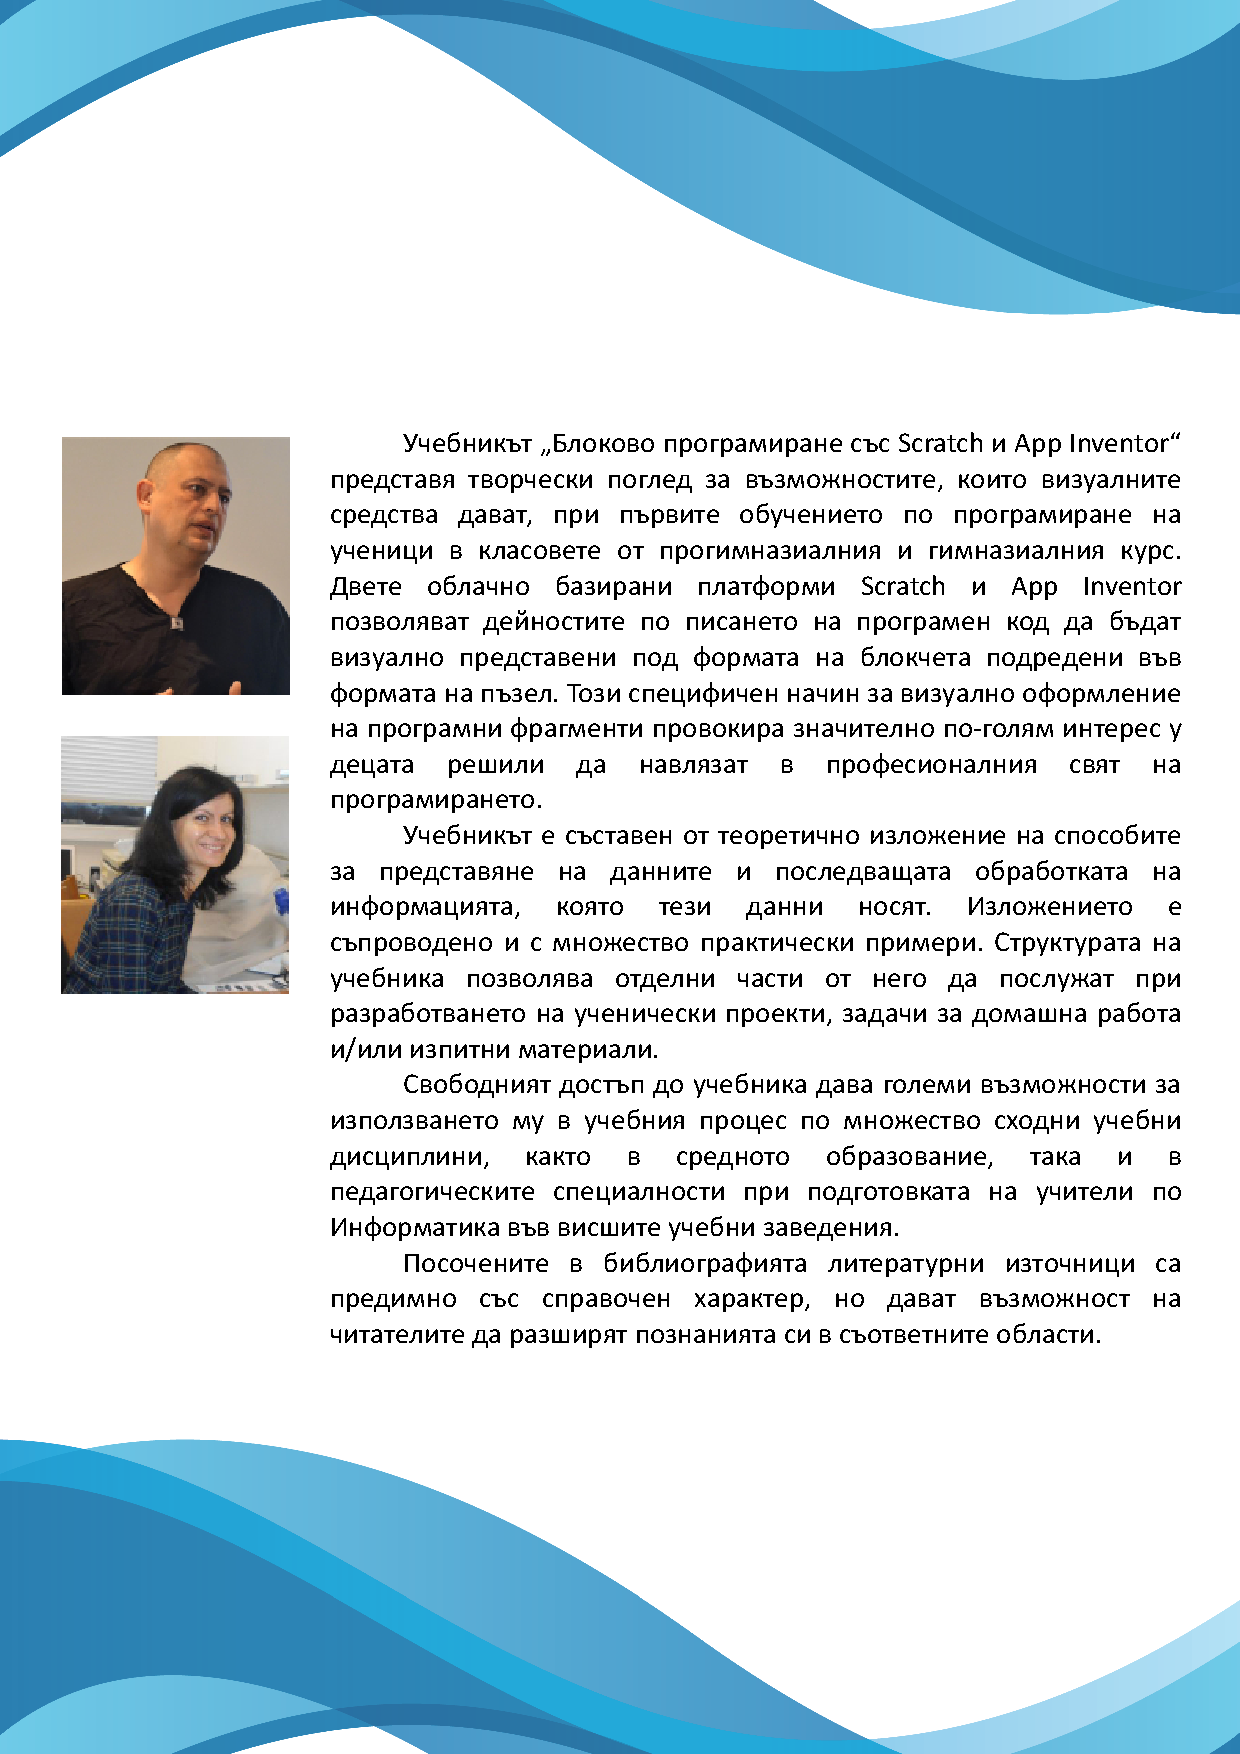
\includepdf[pages=-]{cover/back}

\end{document}